\section{System architecture}
\label{sec:sys_arch}

The developed 4D GIS has a two-tier {\em client-server} architecture
(Figure \ref{fig:sys_arch_2tier}). The {\em server} contains the raw data master
copy and a PostgreSQL database called \textit{viaappiadb}. Both are used
for data preparation. The data preparation occurs at the server and its outcome
is the data set and metadata to be sent to the 4D viewers.

A diagram of the data preparation framework is shown in Figure \ref{fig:sys_arch_data_framework}.
The acquired data for the road itself (background) is usually point clouds,
while for the monuments (sites) the data is of more modalities- point clouds,
meshes, pictures. Depending on the preferred application on the client side,
Windows desktop viewer or Web-based viewer, the raw data is handled differently.

For the Windows desktop viewer the raw data is converted to the OpenSceneGraph
(\url{http://www.openscenegraph.org}) binary format. For the web-base viewer only
point cloud (PC) data is converted and its conversion is done using POTREE (\url{potree.org}) WebGL point
cloud converter. Its output is a octree where each leaf node is a file of format LAS
or LAZ. 

During the data preparation process the \textit{viaappiadb} database is filled with
meta-data information which contains the raw data location and converted data location.
Furthermore, the archaeological information with attribute data for the several sites
is extracted from a Microsoft Access file. The footprints are provided in a PostgreSQL
dump file and are imported into the \textit{viaappiadb} database as well. The altitude
ranges are derived from the PC raw data in combination with the footprints and added
to the Database. On Figures \ref{fig:sys_arch_data_framework} and \ref{fig:sys_arch_2tier}
the solid arrows indicate data flow, while the dashed arrows indicate meta-data flow
during the data preparation process.

\begin{figure}[H] \centering
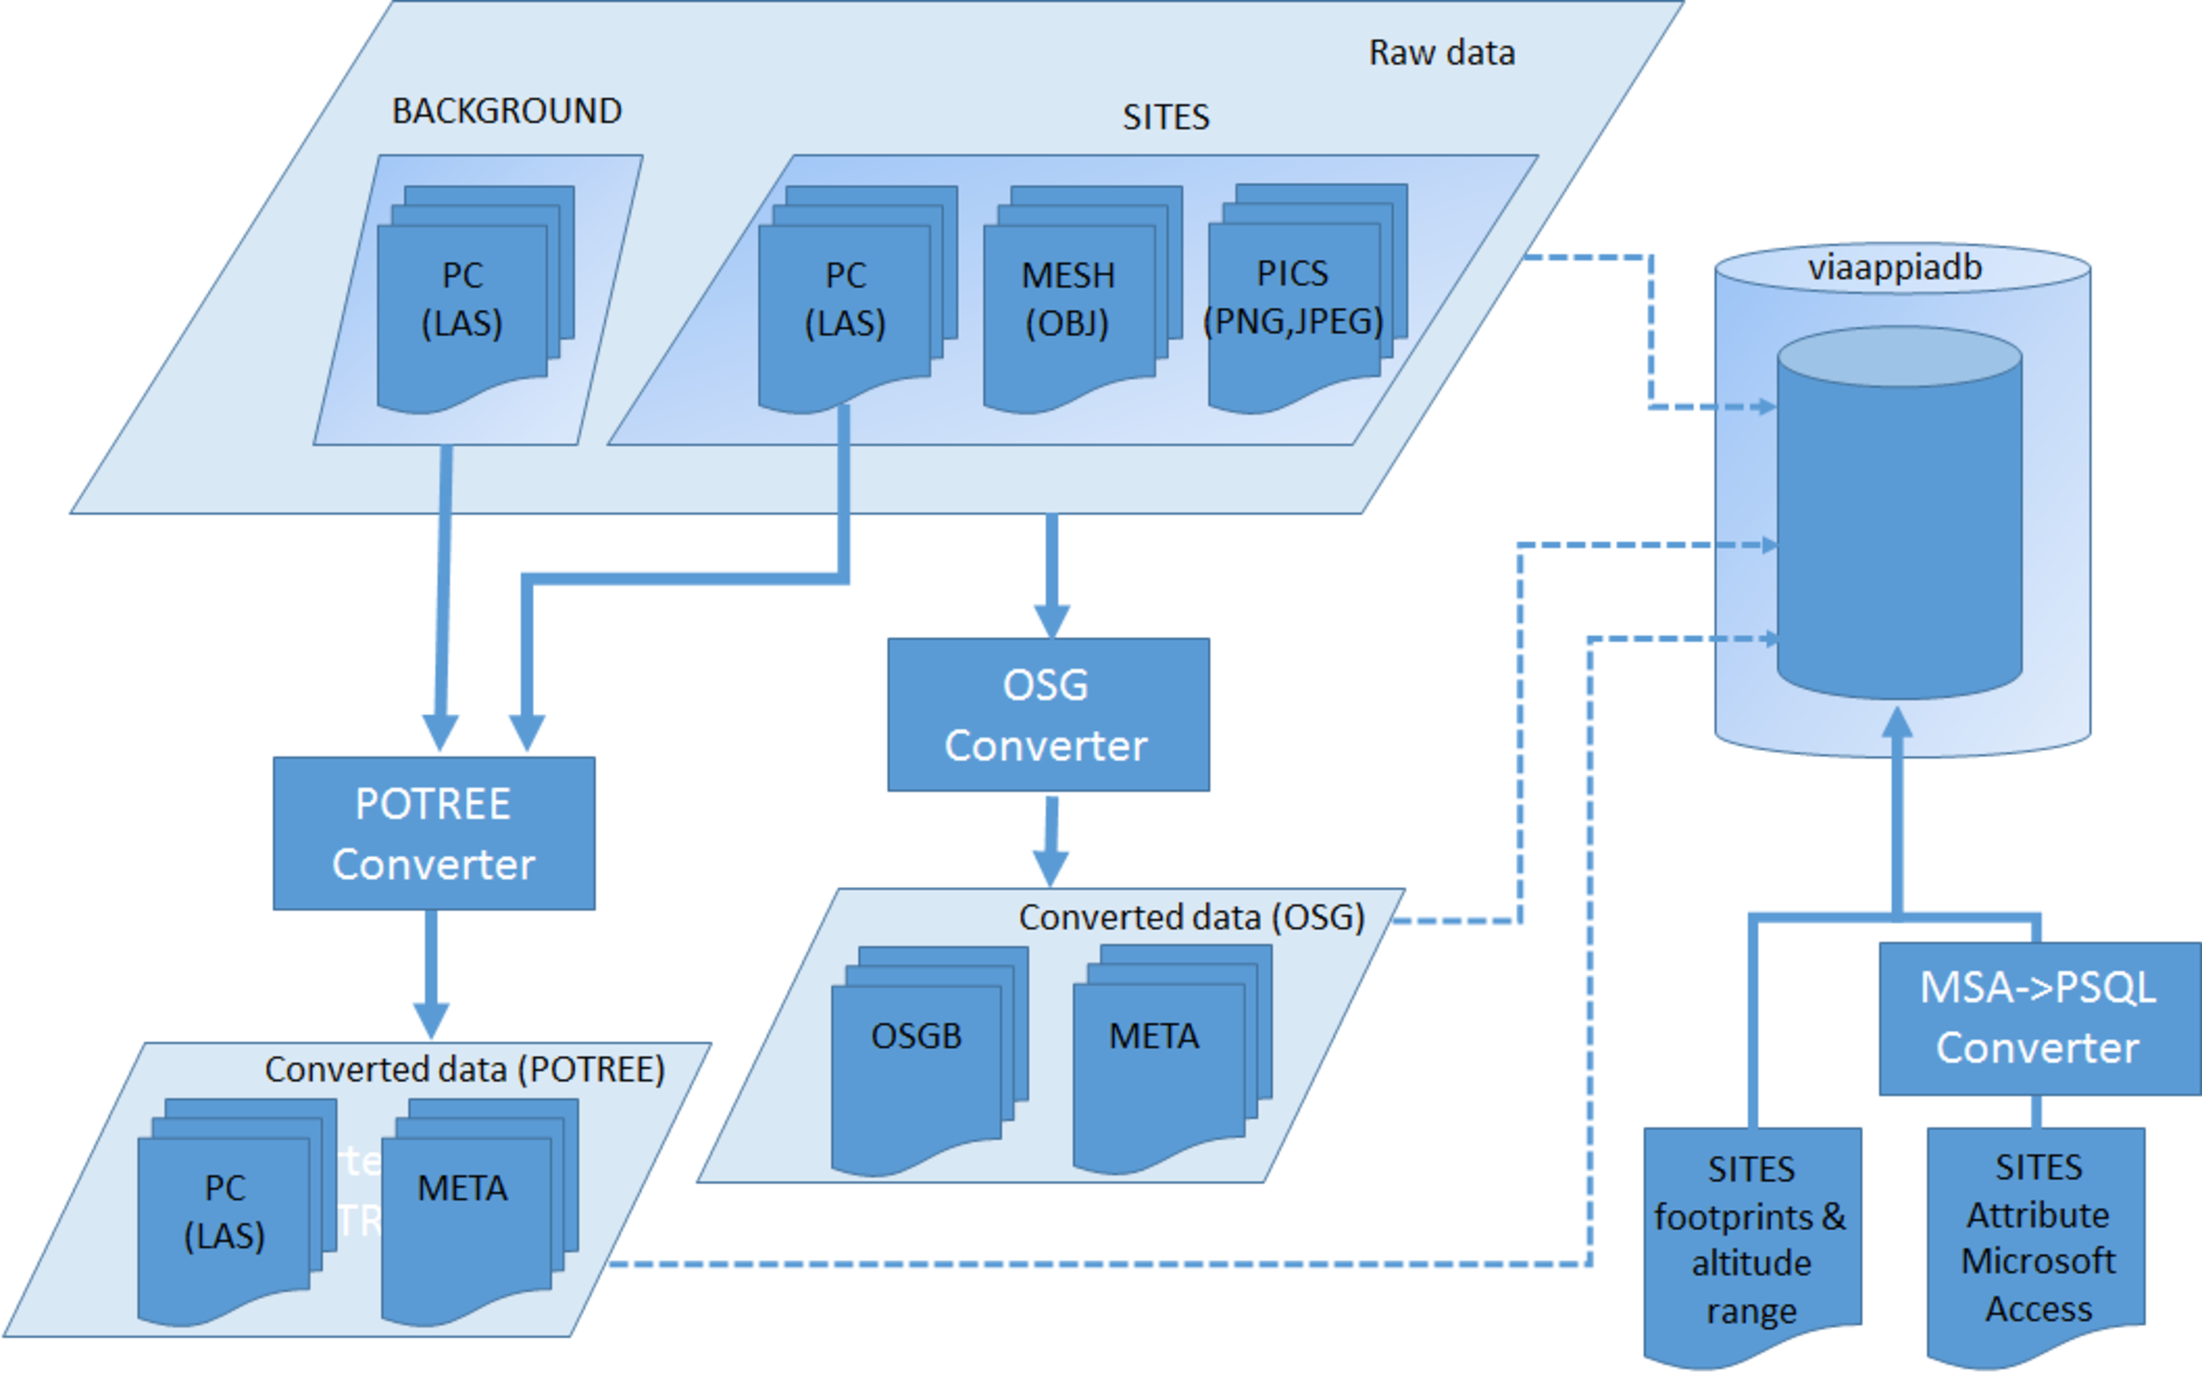
\includegraphics[width=0.75\textwidth]{fig/system_architecture/DataFramework.pdf}
\caption{Data preparation framework executed on the Via Appia Linux serer}
\label{fig:sys_arch_data_framework} \end{figure}

Once the data preparation framework has concluded its task the data is made available
for multi-client sessions. In the case of Windows desktop viewers a local copy of the
entire OSG data set is required before initializing the viewer.

A \textit{launcher} tool based on the Xenon library (\url{http://nlesc.github.io/Xenon/}),
developed by the Netherlands eScience Center (NLeSC), makes sure the local copy is
synchronized with the server. It also retrieves from the server the configuration
file required by the desktop viewer. Once the synchronization finishes the launcher
is in charge of starting the viewer. In the end of a session the launcher updates
the remote database using the modified configuration file. Offline operational
mode is also provided, this is, the user decides when to synchronize.

For the Web-based viewer it is not required a local copy of the entire Potree converted
data set. The necessary data is pulled from the server on request via NGINX Web server
(\url{nginx.com}). Such data also includes a JSON configuration file containing the
meta-data for the background and sites information extracted from the {\em viaappia}
database. The 4D Web-based viewer have been developed by NLeSC. Figure \ref{fig:sys_arch_2tier}
illustrates the two-tier architecture and shows the steps performed at the client
side. 

All the process described so far has been automated. Section~\ref{sec:software} contains
more detailed information about the architecture. 

\begin{figure}[H] \centering
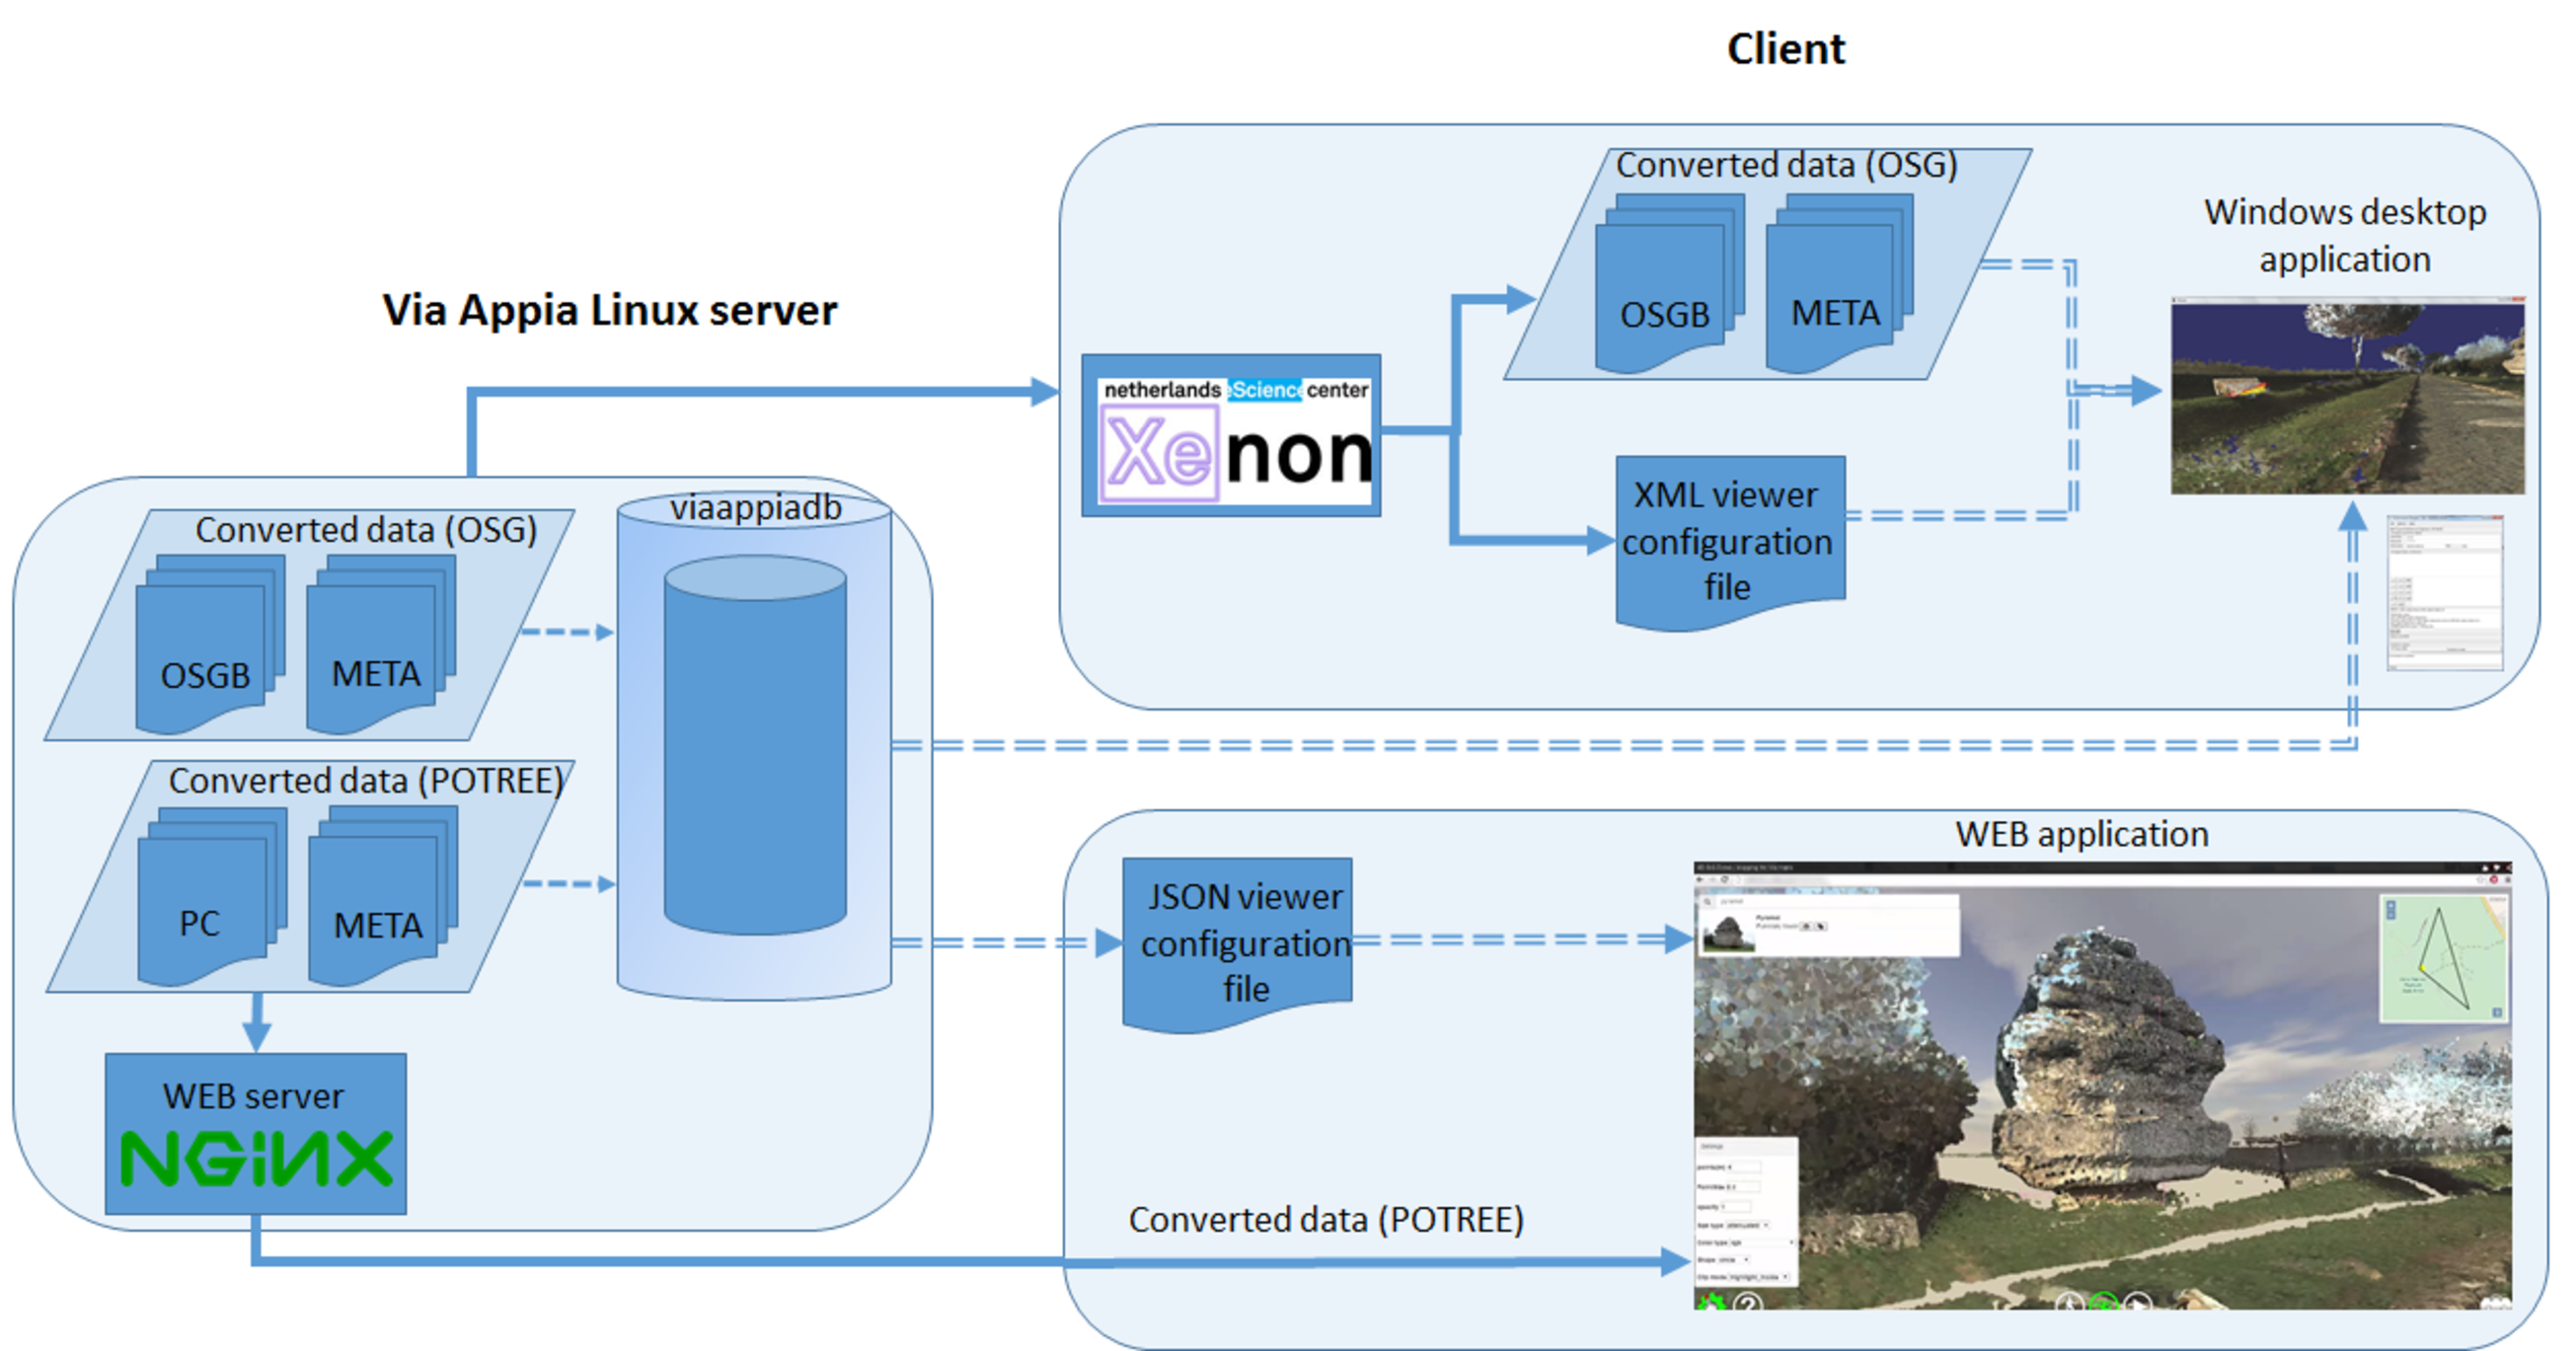
\includegraphics[width=0.95\textwidth]{fig/system_architecture/TwoTierArchitecture.pdf}
\caption{Two-tier architecture of the Via Appia 4D/4D GIS and the steps
executed on the client side.} \label{fig:sys_arch_2tier} \end{figure}
